\documentclass[11pt, a4paper]{article}

% ── Packages ─────────────────────────────────────────────────────────────────
\usepackage[margin=0.75in]{geometry}
\usepackage{graphicx}
\usepackage[table]{xcolor}
\usepackage{titlesec}
\usepackage{enumitem}
\usepackage{booktabs}
\usepackage{longtable}
\usepackage{tabularx}
\usepackage{array}
\usepackage{hyperref}
\usepackage{fancyhdr}
\usepackage{tcolorbox}
\usepackage{fontawesome5}
\usepackage{multicol}
\usepackage{listings}
\usepackage{tikz}
\usepackage{pgfplots}
\usepackage{float}
\usepackage{amsmath}
\usepackage{parskip}

\pgfplotsset{compat=1.18}
\usetikzlibrary{shapes.geometric, arrows.meta, positioning, fit, backgrounds, calc}

% ── Colors (LeadFreak Palette) ───────────────────────────────────────────────
\definecolor{primary}{HTML}{1A1A2E}
\definecolor{secondary}{HTML}{16213E}
\definecolor{accent}{HTML}{0F3460}
\definecolor{highlight}{HTML}{E94560}
\definecolor{success}{HTML}{27AE60}
\definecolor{warning}{HTML}{F39C12}
\definecolor{info}{HTML}{3498DB}
\definecolor{lightbg}{HTML}{F8F9FA}
\definecolor{codebg}{HTML}{1E1E2E}
\definecolor{codetext}{HTML}{CDD6F4}
\definecolor{tableheader}{HTML}{1A1A2E}
\definecolor{tablerow}{HTML}{F0F2F5}
\definecolor{bordergray}{HTML}{DEE2E6}

% ── Heading Styles ───────────────────────────────────────────────────────────
\titleformat{\section}
  {\LARGE\bfseries\color{primary}}
  {\thesection.}{0.5em}{}
  [\vspace{-0.5em}\textcolor{highlight}{\rule{\textwidth}{2pt}}]

\titleformat{\subsection}
  {\Large\bfseries\color{secondary}}
  {\thesubsection}{0.5em}{}

\titleformat{\subsubsection}
  {\large\bfseries\color{accent}}
  {\thesubsubsection}{0.5em}{}

% ── Header / Footer ─────────────────────────────────────────────────────────
\pagestyle{fancy}
\fancyhf{}
\fancyhead[L]{\small\color{accent}\textbf{Fantastic Jobs API Wrapper}}
\fancyhead[R]{\small\color{accent}Technical Documentation}
\fancyfoot[C]{\small\color{accent}\thepage}
\fancyfoot[R]{\small\color{bordergray}Confidential}
\renewcommand{\headrulewidth}{1pt}
\renewcommand{\headrule}{\hbox to\headwidth{\color{highlight}\leaders\hrule height \headrulewidth\hfill}}
\renewcommand{\footrulewidth}{0.5pt}
\renewcommand{\footrule}{\hbox to\headwidth{\color{bordergray}\leaders\hrule height \footrulewidth\hfill}}

% ── Hyperlink Style ──────────────────────────────────────────────────────────
\hypersetup{colorlinks=true, linkcolor=accent, urlcolor=info, citecolor=accent}

% ── Code Listings ────────────────────────────────────────────────────────────
\lstdefinestyle{apistyle}{
    backgroundcolor=\color{codebg},
    basicstyle=\ttfamily\footnotesize\color{codetext},
    breaklines=true, frame=single, rulecolor=\color{bordergray},
    xleftmargin=1em, framexleftmargin=0.5em, numbers=none,
    showstringspaces=false,
    keywordstyle=\color{info}\bfseries,
    stringstyle=\color{success},
    commentstyle=\color{bordergray}\itshape,
}

% ── Custom Boxes ─────────────────────────────────────────────────────────────
\newtcolorbox{infobox}[1][]{colback=info!5, colframe=info, fonttitle=\bfseries, title=#1, arc=3pt, boxrule=1pt, left=6pt, right=6pt}
\newtcolorbox{successbox}[1][]{colback=success!5, colframe=success, fonttitle=\bfseries, title=#1, arc=3pt, boxrule=1pt, left=6pt, right=6pt}
\newtcolorbox{accentbox}[1][]{colback=highlight!5, colframe=highlight, fonttitle=\bfseries, title=#1, arc=3pt, boxrule=1pt, left=6pt, right=6pt}
\newtcolorbox{warnbox}[1][]{colback=warning!5, colframe=warning, fonttitle=\bfseries, title=#1, arc=3pt, boxrule=1pt, left=6pt, right=6pt}

% ── Column Types ─────────────────────────────────────────────────────────────
\newcolumntype{L}[1]{>{\raggedright\arraybackslash}p{#1}}
\newcolumntype{C}[1]{>{\centering\arraybackslash}p{#1}}
\newcolumntype{R}[1]{>{\raggedleft\arraybackslash}p{#1}}

% ── Check / Cross marks ─────────────────────────────────────────────────────
\newcommand{\cmark}{\textcolor{success}{\faCheck}}
\newcommand{\xmark}{\textcolor{highlight}{\faTimes}}

% ══════════════════════════════════════════════════════════════════════════════
\begin{document}

% ── Title Page ───────────────────────────────────────────────────────────────
\begin{titlepage}
\begin{tikzpicture}[remember picture, overlay]
    \fill[primary] (current page.south west) rectangle (current page.north east);
    \fill[highlight] ([yshift=-4cm]current page.north west) rectangle ([yshift=-4.15cm]current page.north east);
    \fill[accent] (current page.south west) rectangle ([yshift=3cm]current page.south east);
    \foreach \i in {1,...,8} {
        \fill[white, opacity=0.03] ([xshift=\i*2cm, yshift=-8cm]current page.north west) circle (3cm);
    }
\end{tikzpicture}
\vspace*{3cm}
\begin{center}
    {\fontsize{42}{50}\selectfont\bfseries\color{white}Fantastic Jobs}\\[0.3cm]
    {\fontsize{42}{50}\selectfont\bfseries\color{highlight}API Wrapper}\\[1.5cm]
    {\LARGE\color{white!80}Technical Architecture \&}\\[0.2cm]
    {\LARGE\color{white!80}Implementation Document}\\[0.5cm]
    \textcolor{highlight}{\rule{8cm}{2pt}}\\[2cm]
    {\large\color{white!70}
    \begin{tabular}{rl}
        \textbf{\color{white}Version:} & 1.0.0 \\[0.3cm]
        \textbf{\color{white}Date:} & March 28, 2026 \\[0.3cm]
        \textbf{\color{white}Stack:} & FastAPI + RapidAPI \\[0.3cm]
        \textbf{\color{white}Status:} & Implementation Complete \\
    \end{tabular}}
\end{center}
\vfill
\begin{center}
    {\small\color{white!50}Confidential -- Internal Use Only}
\end{center}
\end{titlepage}

\newpage
\tableofcontents
\newpage

% ══════════════════════════════════════════════════════════════════════════════
\section{Executive Summary}
% ══════════════════════════════════════════════════════════════════════════════

\begin{accentbox}[\faRocket\hspace{0.5em} What We Built]
A \textbf{FastAPI wrapper API} that takes job titles (directly or from stored client config) and queries the \textbf{Fantastic Jobs APIs} (via RapidAPI) to fetch, filter, normalize, and serve enriched job listing data from \textbf{175,000+ career sites} and \textbf{LinkedIn}. On-demand only --- you hit it when you need fresh jobs.
\end{accentbox}

\subsection{Two Separate APIs}

\begin{center}
\small
\begin{tabularx}{\textwidth}{|C{1.5cm}|L{3.5cm}|X|}
\hline
\rowcolor{tableheader}
\textcolor{white}{\textbf{\#}} & \textcolor{white}{\textbf{API}} & \textcolor{white}{\textbf{Purpose}} \\
\hline
1 & \textbf{Job Roles API} (external, existing) & Called \textbf{once} during client onboarding. Returns job titles/roles. Output stored in our DB. \\
\rowcolor{tablerow}
2 & \textbf{Job Search API} (this project) & Called \textbf{on-demand} whenever you want fresh jobs. Uses stored roles or directly provided titles. \\
\hline
\end{tabularx}
\end{center}

\subsection{Solution Overview}

\begin{center}
\begin{tikzpicture}[
    node distance=1cm and 1.5cm,
    box/.style={rectangle, rounded corners=5pt, draw=accent, fill=lightbg, minimum width=2.6cm, minimum height=1cm, align=center, font=\footnotesize\bfseries, text=primary},
    apibox/.style={rectangle, rounded corners=5pt, draw=highlight, fill=highlight!10, minimum width=2.6cm, minimum height=1cm, align=center, font=\footnotesize\bfseries, text=primary},
    dbbox/.style={cylinder, draw=success, fill=success!10, minimum width=2cm, minimum height=0.8cm, align=center, font=\footnotesize\bfseries, text=primary, shape border rotate=90, aspect=0.3},
    arr/.style={-{Stealth[length=2.5mm]}, thick, color=accent},
]
    \node[box] (roles) {\faCode~Job Roles\\API (once)};
    \node[dbbox, right=of roles] (db) {Client DB\\(roles+filters)};
    \node[box, right=of db] (wrapper) {\faCogs~Job Search\\API (FastAPI)};
    \node[apibox, above right=0.6cm and 1.5cm of wrapper] (ats) {\faBriefcase~ATS API};
    \node[apibox, below right=0.6cm and 1.5cm of wrapper] (li) {\faLinkedin~LinkedIn API};

    \draw[arr] (roles) -- node[above, font=\scriptsize\color{accent}] {onboard} (db);
    \draw[arr] (db) -- node[above, font=\scriptsize\color{accent}] {roles} (wrapper);
    \draw[arr] (wrapper) -- node[above, sloped, font=\scriptsize\color{accent}] {query} (ats);
    \draw[arr] (wrapper) -- node[below, sloped, font=\scriptsize\color{accent}] {query} (li);
    \draw[arr] (ats) -- node[above, sloped, font=\scriptsize\color{highlight}] {jobs} (wrapper);
    \draw[arr] (li) -- node[below, sloped, font=\scriptsize\color{highlight}] {jobs} (wrapper);
\end{tikzpicture}
\end{center}

\subsection{Key Metrics}

\begin{center}
\small
\begin{tabularx}{\textwidth}{|X|X|X|X|}
\hline
\rowcolor{tableheader}
\textcolor{white}{\textbf{Career Sites}} & \textcolor{white}{\textbf{ATS Platforms}} & \textcolor{white}{\textbf{Jobs/Month}} & \textcolor{white}{\textbf{API Parameters}} \\
\hline
\centering 175,000+ & \centering 54 & \centering 10M+ & \centering\arraybackslash 50+ \\
\hline
\end{tabularx}
\end{center}

% ══════════════════════════════════════════════════════════════════════════════
\newpage
\section{Upstream APIs -- Fantastic Jobs (RapidAPI)}
% ══════════════════════════════════════════════════════════════════════════════

We integrate with \textbf{two} Fantastic Jobs APIs on RapidAPI. The user chooses which to query via the \texttt{source} parameter.

\subsection{API 1: Active Jobs DB (ATS / Career Sites)}

\begin{infobox}[\faBriefcase\hspace{0.5em} ATS API Overview]
\small
\begin{tabular}{@{}l@{\hspace{1em}}l@{}}
    \textbf{RapidAPI Host:} & \texttt{active-jobs-db.p.rapidapi.com} \\
    \textbf{Data Source:} & 175,000+ employer career sites \\
    \textbf{ATS Platforms:} & 54 (Workday, Greenhouse, Lever, Ashby, etc.) \\
    \textbf{Volume:} & 2.5M+ jobs/month \\
    \textbf{Refresh Rate:} & Hourly (95\% within 3 hours of posting) \\
    \textbf{Backfill:} & Up to 6 months of historical data \\
\end{tabular}
\end{infobox}

\subsubsection{ATS Endpoints}

\begin{center}\small
\begin{tabularx}{\textwidth}{|L{3.5cm}|L{3.5cm}|X|}
\hline
\rowcolor{tableheader}
\textcolor{white}{\textbf{Endpoint}} & \textcolor{white}{\textbf{Path}} & \textcolor{white}{\textbf{Use Case}} \\
\hline
Active Jobs 7 Days & \texttt{/active-ats-7d} & Weekly batch, default \\
\rowcolor{tablerow}
Active Jobs 24 Hours & \texttt{/active-ats-24h} & Daily fresh jobs \\
Hourly Feed & \texttt{/active-ats-1h} & Real-time ingestion \\
\rowcolor{tablerow}
Expired Jobs & \texttt{/expired-ats} & Cleanup removed listings \\
Backfill 6 Months & \texttt{/active-ats-6m} & Historical population \\
\hline
\end{tabularx}
\end{center}

\subsubsection{Supported ATS Platforms (54)}

\begin{multicols}{3}
\begin{itemize}[leftmargin=1em, itemsep=0pt, parsep=0pt]
\scriptsize
    \item ADP \item ApplicantPro \item Ashby \item BambooHR \item Breezy
    \item CareerPlug \item Comeet \item CSOD \item Dayforce \item Dover
    \item Eightfold \item FirstStage \item Freshteam \item Gem \item GoHire
    \item Greenhouse \item HiBob \item HireBridge \item HireHive \item Hireology
    \item HiringThing \item iCIMS \item iSolved \item JazzHR \item Jobvite
    \item Join.com \item Kula \item Lever.co \item Manatal \item OracleCloud
    \item PageUp \item Paradox \item Paycom \item Paycor \item Paylocity
    \item Personio \item PhenomPeople \item Pinpoint \item Polymer \item Recruitee
    \item Recooty \item Rippling \item Rival \item SmartRecruiters
    \item SuccessFactors \item Taleo \item Teamtailor \item Trakstar
    \item TriNet \item UltiPro \item WeRecruit \item Workable \item Workday \item Zoho
\end{itemize}
\end{multicols}

\subsection{API 2: LinkedIn Job Search API}

\begin{infobox}[\faLinkedin\hspace{0.5em} LinkedIn API Overview]
\small
\begin{tabular}{@{}l@{\hspace{1em}}l@{}}
    \textbf{RapidAPI Host:} & \texttt{linkedin-job-search-api.p.rapidapi.com} \\
    \textbf{Data Source:} & LinkedIn job postings \\
    \textbf{Volume:} & 9M+ jobs/month, 2M+ weekly \\
    \textbf{Refresh Rate:} & Hourly \\
    \textbf{Special:} & External Apply URLs, Recruiter Details \\
\end{tabular}
\end{infobox}

\subsubsection{LinkedIn Endpoints}

\begin{center}\small
\begin{tabularx}{\textwidth}{|L{3cm}|L{4.5cm}|X|}
\hline
\rowcolor{tableheader}
\textcolor{white}{\textbf{Endpoint}} & \textcolor{white}{\textbf{Path}} & \textcolor{white}{\textbf{Use Case}} \\
\hline
Active 7 Days & \texttt{/active-jb-7d} & Weekly batch, default \\
\rowcolor{tablerow}
Active 24 Hours & \texttt{/active-jb-24h} & Daily / description search \\
Backfill 6M & \texttt{/active-jb-6m} & Historical data \\
\rowcolor{tablerow}
Ultra Hourly & \texttt{/ultra/active-jb-1h} & Real-time feed \\
Ultra Expired & \texttt{/ultra/expired-jb} & Cleanup \\
\hline
\end{tabularx}
\end{center}

\subsection{Key Differences Between APIs}

\begin{center}\small
\begin{tabularx}{\textwidth}{|L{3.8cm}|X|X|}
\hline
\rowcolor{tableheader}
\textcolor{white}{\textbf{Feature}} & \textcolor{white}{\textbf{ATS API}} & \textcolor{white}{\textbf{LinkedIn API}} \\
\hline
Experience entry level & \texttt{0-2} & \texttt{0-3} \\
\rowcolor{tablerow}
ATS platform filter & \cmark~\texttt{source} & \xmark \\
Seniority filter & \xmark & \cmark~\texttt{seniority\_filter} \\
\rowcolor{tablerow}
Job type filter & AI only & \cmark~\texttt{type\_filter} \\
Dedup with other API & \xmark & \cmark \\
\rowcolor{tablerow}
EasyApply filter & \xmark & \cmark~\texttt{directApply} \\
Adv.\ description filter & \cmark & \xmark \\
\rowcolor{tablerow}
Sort order & \xmark & \cmark~\texttt{order} \\
Desc.\ filter timeout & No risk & Risk on 7d endpoint \\
\hline
\end{tabularx}
\end{center}

% ══════════════════════════════════════════════════════════════════════════════
\newpage
\section{Complete Parameter Reference}
% ══════════════════════════════════════════════════════════════════════════════

\subsection{Shared Parameters (Both APIs)}

{\footnotesize
\begin{longtable}{|L{5.2cm}|C{1.2cm}|C{1.2cm}|L{7cm}|}
\hline
\rowcolor{tableheader}
\textcolor{white}{\textbf{Parameter}} & \textcolor{white}{\textbf{Type}} & \textcolor{white}{\textbf{Default}} & \textcolor{white}{\textbf{Description}} \\
\hline
\endfirsthead
\hline
\rowcolor{tableheader}
\textcolor{white}{\textbf{Parameter}} & \textcolor{white}{\textbf{Type}} & \textcolor{white}{\textbf{Default}} & \textcolor{white}{\textbf{Description}} \\
\hline
\endhead

\texttt{limit} & Number & 100 & Jobs per call (10--100) \\
\rowcolor{tablerow}
\texttt{offset} & Number & 0 & Pagination offset \\
\texttt{title\_filter} & String & -- & Google-style title search \\
\rowcolor{tablerow}
\texttt{advanced\_title\_filter} & String & -- & Operators: \texttt{\& | ! <-> :*}. Cannot combine with \texttt{title\_filter} \\
\texttt{location\_filter} & String & -- & Full names, \texttt{OR} for multiple \\
\rowcolor{tablerow}
\texttt{organization\_filter} & String & -- & Exact match, comma-delimited \\
\texttt{organization\_exclusion\_filter} & String & -- & Exclude orgs, comma-delimited \\
\rowcolor{tablerow}
\texttt{advanced\_organization\_filter} & String & -- & Same operators as title \\
\texttt{description\_type} & String & \texttt{text} & \texttt{text}, \texttt{html}, or empty \\
\rowcolor{tablerow}
\texttt{remote} & Bool & -- & \texttt{true}/\texttt{false}/empty \\
\texttt{agency} & Bool & -- & \texttt{TRUE}=agencies only \\
\rowcolor{tablerow}
\texttt{date\_filter} & String & -- & Greater-than date. UTC. \\
\texttt{include\_ai} & Bool & \texttt{true}* & Enable AI-enriched fields \\
\rowcolor{tablerow}
\texttt{include\_li} & Bool & \texttt{true}* & LinkedIn company profiles \\
\texttt{ai\_employment\_type\_filter} & String & -- & FULL\_TIME, PART\_TIME, etc. \\
\rowcolor{tablerow}
\texttt{ai\_work\_arrangement\_filter} & String & -- & On-site, Hybrid, Remote OK/Solely \\
\texttt{ai\_has\_salary} & Bool & -- & Only jobs with salary data \\
\rowcolor{tablerow}
\texttt{ai\_visa\_sponsorship\_filter} & Bool & -- & Jobs mentioning visa \\
\texttt{ai\_taxonomies\_a\_filter} & String & -- & 33 categories (Technology, etc.) \\
\rowcolor{tablerow}
\texttt{ai\_taxonomies\_a\_primary\_filter} & String & -- & Primary taxonomy only \\
\texttt{ai\_taxonomies\_a\_exclusion\_filter} & String & -- & Exclude taxonomies \\
\rowcolor{tablerow}
\texttt{li\_organization\_slug\_filter} & String & -- & LinkedIn company slug \\
\texttt{li\_organization\_slug\_exclusion\_filter} & String & -- & Exclude company slugs \\
\rowcolor{tablerow}
\texttt{li\_industry\_filter} & String & -- & Exact, case-sensitive \\
\texttt{li\_organization\_specialties\_filter} & String & -- & Company specialties search \\
\rowcolor{tablerow}
\texttt{li\_organization\_description\_filter} & String & -- & Company description search \\
\texttt{li\_organization\_employees\_lte} & Number & -- & Max employees \\
\rowcolor{tablerow}
\texttt{li\_organization\_employees\_gte} & Number & -- & Min employees \\
\hline
\end{longtable}
}
{\small * Smart defaults set by our wrapper}

\subsection{ATS-Only Parameters}

\begin{center}\small
\begin{tabularx}{\textwidth}{|L{4.5cm}|C{1.5cm}|X|}
\hline
\rowcolor{tableheader}
\textcolor{white}{\textbf{Parameter}} & \textcolor{white}{\textbf{Type}} & \textcolor{white}{\textbf{Description}} \\
\hline
\texttt{description\_filter} & String & Google-style description search \\
\rowcolor{tablerow}
\texttt{advanced\_description\_filter} & String & Advanced operators on description \\
\texttt{source} & String & ATS platform filter (54 options) \\
\rowcolor{tablerow}
\texttt{source\_exclusion} & String & Exclude ATS platforms \\
\texttt{ai\_experience\_level\_filter} & String & \texttt{0-2}, \texttt{2-5}, \texttt{5-10}, \texttt{10+} \\
\hline
\end{tabularx}
\end{center}

\subsection{LinkedIn-Only Parameters}

\begin{center}\small
\begin{tabularx}{\textwidth}{|L{4.5cm}|C{1.5cm}|X|}
\hline
\rowcolor{tableheader}
\textcolor{white}{\textbf{Parameter}} & \textcolor{white}{\textbf{Type}} & \textcolor{white}{\textbf{Description}} \\
\hline
\texttt{description\_filter} & String & Risky on 7d (auto-switches to 24h) \\
\rowcolor{tablerow}
\texttt{organization\_description\_filter} & String & LinkedIn org description \\
\texttt{organization\_specialties\_filter} & String & LinkedIn org specialties \\
\rowcolor{tablerow}
\texttt{organization\_slug\_filter} & String & Company slug, exact match \\
\texttt{type\_filter} & String & FULL\_TIME, PART\_TIME, INTERN, etc. \\
\rowcolor{tablerow}
\texttt{seniority\_filter} & String & Associate, Director, Executive, etc. \\
\texttt{exclude\_ats\_duplicate} & Bool & Auto-set when \texttt{source=both} \\
\rowcolor{tablerow}
\texttt{external\_apply\_url} & Bool & Only with external apply URL \\
\texttt{directApply} & Bool & Include/exclude EasyApply \\
\rowcolor{tablerow}
\texttt{employees\_lte / \_gte} & Number & Company size filter (native) \\
\texttt{order} & String & \texttt{desc} (default) or \texttt{asc} \\
\rowcolor{tablerow}
\texttt{ai\_experience\_level\_filter} & String & \texttt{0-3}, \texttt{2-5}, \texttt{5-10}, \texttt{10+} \\
\hline
\end{tabularx}
\end{center}

% ══════════════════════════════════════════════════════════════════════════════
\newpage
\section{Our Wrapper API -- Architecture}
% ══════════════════════════════════════════════════════════════════════════════

\subsection{Tech Stack}

\begin{center}\small
\begin{tabularx}{\textwidth}{|L{2.8cm}|L{3.5cm}|X|}
\hline
\rowcolor{tableheader}
\textcolor{white}{\textbf{Layer}} & \textcolor{white}{\textbf{Technology}} & \textcolor{white}{\textbf{Purpose}} \\
\hline
Framework & FastAPI & Async REST API with auto-docs \\
\rowcolor{tablerow}
HTTP Client & httpx & Async HTTP calls to RapidAPI \\
Database & SQLite / PostgreSQL & Client configs (job\_roles + filters) \\
\rowcolor{tablerow}
Validation & Pydantic v2 & Request/response schemas, enums \\
Retry & tenacity & Exponential backoff on failures \\
\rowcolor{tablerow}
Rate Limit & asyncio.Semaphore & Concurrent request capping \\
Logging & Custom (on/off via .env) & Full request/response tracing \\
\hline
\end{tabularx}
\end{center}

\subsection{Project Structure}

\begin{lstlisting}[style=apistyle]
fantastic-jobs-api/
|-- app/
|   |-- main.py                    # FastAPI app + lifespan
|   |-- core/
|   |   |-- config.py              # Settings (pydantic-settings)
|   |   |-- exceptions.py          # Custom HTTP exceptions
|   |   |-- logging_config.py      # Colored logging (on/off via .env)
|   |-- db/
|   |   |-- base.py, session.py    # SQLAlchemy async setup
|   |   |-- models.py              # ClientConfig (job_roles, filters)
|   |-- schemas/
|   |   |-- common.py              # Enums, pagination, constants
|   |   |-- filters.py             # SharedFilters, ATSFilters, LinkedInFilters
|   |   |-- request.py             # JobSearchRequest
|   |   |-- response.py            # NormalizedJob, SearchResponse
|   |   |-- client_config.py       # Client onboarding schemas
|   |-- api/v1/endpoints/
|   |   |-- search.py              # POST /search
|   |   |-- clients.py             # Client onboarding CRUD
|   |-- services/
|       |-- query_builder.py       # Title -> filter (if-else logic)
|       |-- ats_client.py          # ATS API HTTP client
|       |-- linkedin_client.py     # LinkedIn API HTTP client
|       |-- normalizer.py          # Response normalization
|       |-- search_orchestrator.py # Central coordination
|-- .env, requirements.txt
\end{lstlisting}

\subsection{API Endpoints}

\begin{center}\small
\begin{tabularx}{\textwidth}{|C{1.3cm}|L{4.5cm}|X|}
\hline
\rowcolor{tableheader}
\textcolor{white}{\textbf{Method}} & \textcolor{white}{\textbf{Path}} & \textcolor{white}{\textbf{Description}} \\
\hline
POST & \texttt{/api/v1/search} & Search jobs (titles directly or via client\_id) \\
\rowcolor{tablerow}
POST & \texttt{/api/v1/clients/} & Onboard client (store job\_roles + filters) \\
GET & \texttt{/api/v1/clients/\{id\}} & Read client config \\
\rowcolor{tablerow}
PUT & \texttt{/api/v1/clients/\{id\}} & Update client config / job\_roles \\
DELETE & \texttt{/api/v1/clients/\{id\}} & Delete client \\
\rowcolor{tablerow}
GET & \texttt{/health} & Health check \\
\hline
\end{tabularx}
\end{center}

% ══════════════════════════════════════════════════════════════════════════════
\section{Query Building Logic}
% ══════════════════════════════════════════════════════════════════════════════

Pure if-else logic, no LLM. The \texttt{query\_builder.py} converts titles into API filter expressions:

\begin{center}\small
\begin{tabularx}{\textwidth}{|L{4.5cm}|L{3cm}|X|}
\hline
\rowcolor{tableheader}
\textcolor{white}{\textbf{Input Titles}} & \textcolor{white}{\textbf{Filter Used}} & \textcolor{white}{\textbf{Generated Expression}} \\
\hline
\texttt{["Data Engineer"]} & \texttt{title\_filter} & \texttt{"Data Engineer"} \\
\rowcolor{tablerow}
\texttt{["Software Engineer", "Backend Developer"]} & \texttt{advanced\_title\_filter} & \texttt{'Software Engineer' | 'Backend Developer'} \\
\texttt{["ML Engineer", "AI Researcher", "Data Scientist"]} & \texttt{advanced\_title\_filter} & \texttt{'ML Engineer' | 'AI Researcher' | 'Data Scientist'} \\
\hline
\end{tabularx}
\end{center}

\textbf{Rules:}
\begin{itemize}[leftmargin=1.5em, itemsep=2pt]
    \item \textbf{1 title} $\rightarrow$ \texttt{title\_filter} with double quotes (Google-style)
    \item \textbf{Multiple titles} $\rightarrow$ \texttt{advanced\_title\_filter} with \texttt{|} (OR), each multi-word title single-quoted
    \item \textbf{Explicit override} $\rightarrow$ if user passes \texttt{title\_filter} or \texttt{advanced\_title\_filter} directly, that wins
\end{itemize}

% ══════════════════════════════════════════════════════════════════════════════
\section{Smart Features}
% ══════════════════════════════════════════════════════════════════════════════

\subsection{Client Onboarding Flow}

\begin{center}
\begin{tikzpicture}[
    node distance=0.6cm and 2cm,
    step/.style={rectangle, rounded corners=4pt, draw=accent, fill=lightbg, text width=0.85\textwidth, minimum height=0.7cm, align=left, font=\footnotesize, text=primary, inner xsep=8pt, inner ysep=4pt},
    arr/.style={-{Stealth[length=2mm]}, thick, color=highlight},
]
    \node[step, fill=highlight!10, draw=highlight] (s1) {\textbf{1.} Call Job Roles API (external) $\rightarrow$ get titles like \texttt{["Data Engineer", "ML Engineer"]}};
    \node[step, below=of s1] (s2) {\textbf{2.} \texttt{POST /api/v1/clients/} with \texttt{job\_roles} + default filters (location, remote, etc.)};
    \node[step, below=of s2, fill=success!10, draw=success] (s3) {\textbf{3.} Client stored in DB. Now just send \texttt{\{"client\_id": "acme"\}} to search.};
    \draw[arr] (s1) -- (s2);
    \draw[arr] (s2) -- (s3);
\end{tikzpicture}
\end{center}

\subsection{Title Resolution}

\begin{center}\small
\begin{tabularx}{\textwidth}{|L{5cm}|X|}
\hline
\rowcolor{tableheader}
\textcolor{white}{\textbf{Request}} & \textcolor{white}{\textbf{Titles Used}} \\
\hline
\texttt{\{"titles": ["PM"]\}} & Directly uses \texttt{["PM"]} \\
\rowcolor{tablerow}
\texttt{\{"client\_id": "acme"\}} & Picks stored \texttt{job\_roles} from DB \\
\texttt{\{"titles": ["PM"], "client\_id": "acme"\}} & Uses \texttt{["PM"]} (explicit override wins) \\
\rowcolor{tablerow}
\texttt{\{"source": "ats"\}} (no titles, no client) & \textbf{422 error} \\
\hline
\end{tabularx}
\end{center}

\subsection{Auto-Deduplication (source = ``both'')}

\begin{infobox}[\faClone\hspace{0.5em} When source = "both"]
\begin{enumerate}[leftmargin=1.5em, itemsep=2pt]
    \item Both API calls execute in \textbf{parallel} via \texttt{asyncio.gather()}
    \item \texttt{exclude\_ats\_duplicate=true} is \textbf{auto-set} on the LinkedIn call
    \item Secondary dedup: hash of \texttt{title + org + location}
\end{enumerate}
\end{infobox}

\subsection{Smart Defaults}

\begin{center}\small
\begin{tabularx}{\textwidth}{|L{3.5cm}|C{2.5cm}|X|}
\hline
\rowcolor{tableheader}
\textcolor{white}{\textbf{Parameter}} & \textcolor{white}{\textbf{Default}} & \textcolor{white}{\textbf{Rationale}} \\
\hline
\texttt{include\_ai} & \texttt{true} & Max data enrichment \\
\rowcolor{tablerow}
\texttt{include\_li} & \texttt{true} & LinkedIn company data always useful \\
\texttt{description\_type} & \texttt{text} & Safe default, lower bandwidth \\
\rowcolor{tablerow}
LinkedIn endpoint & Auto-switch to 24h & When \texttt{description\_filter} used \\
\hline
\end{tabularx}
\end{center}

\subsection{Client Config Merging}

\begin{center}
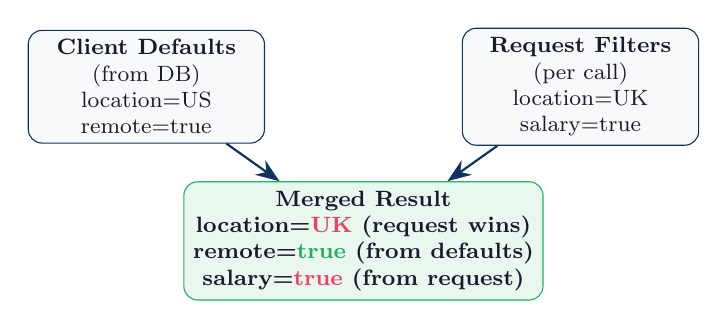
\begin{tikzpicture}[
    box/.style={rectangle, rounded corners=5pt, draw=accent, fill=lightbg, minimum width=3cm, minimum height=1.3cm, align=center, font=\footnotesize, text=primary},
    result/.style={rectangle, rounded corners=5pt, draw=success, fill=success!10, minimum width=3.5cm, minimum height=1.3cm, align=center, font=\footnotesize\bfseries, text=primary},
    arr/.style={-{Stealth[length=3mm]}, thick, color=accent},
]
    \node[box] (client) {\textbf{Client Defaults}\\(from DB)\\location=US\\remote=true};
    \node[box, right=2.5cm of client] (request) {\textbf{Request Filters}\\(per call)\\location=UK\\salary=true};
    \node[result, below=1.2cm of $(client)!0.5!(request)$] (merged) {\textbf{Merged Result}\\location=\textcolor{highlight}{UK} (request wins)\\remote=\textcolor{success}{true} (from defaults)\\salary=\textcolor{highlight}{true} (from request)};
    \draw[arr] (client) -- (merged);
    \draw[arr] (request) -- (merged);
\end{tikzpicture}
\end{center}

\textbf{Rule:} Request-level values \textbf{always override} client defaults. Defaults only fill in unset fields.

% ══════════════════════════════════════════════════════════════════════════════
\section{Response Schema -- NormalizedJob}
% ══════════════════════════════════════════════════════════════════════════════

Both API responses are normalized into a \textbf{unified schema} with 30+ fields:

{\small
\begin{center}
\begin{tabularx}{\textwidth}{|L{3.5cm}|C{1.5cm}|X|}
\hline
\rowcolor{tableheader}
\textcolor{white}{\textbf{Field}} & \textcolor{white}{\textbf{Type}} & \textcolor{white}{\textbf{Description}} \\
\hline
\multicolumn{3}{|l|}{\cellcolor{accent!10}\textbf{\color{accent}Core Fields}} \\
\hline
\texttt{id} & String & Unique job ID from source \\
\rowcolor{tablerow}
\texttt{title} & String & Job title \\
\texttt{organization} & String & Company name \\
\rowcolor{tablerow}
\texttt{location} & String & Full location string \\
\texttt{url} & String & Apply / posting URL \\
\rowcolor{tablerow}
\texttt{source\_api} & Enum & \texttt{"ats"} or \texttt{"linkedin"} \\
\texttt{source\_platform} & String & ATS name or \texttt{"linkedin"} \\
\rowcolor{tablerow}
\texttt{date\_posted} & String & Posting date (UTC) \\
\hline
\multicolumn{3}{|l|}{\cellcolor{accent!10}\textbf{\color{accent}Location Details}} \\
\hline
\texttt{city / state / country} & String & Parsed location components \\
\rowcolor{tablerow}
\texttt{is\_remote} & Boolean & Remote job flag \\
\hline
\multicolumn{3}{|l|}{\cellcolor{accent!10}\textbf{\color{accent}Salary}} \\
\hline
\texttt{salary\_raw} & String & Raw salary string \\
\rowcolor{tablerow}
\texttt{ai\_salary\_min/max} & Float & AI-extracted range \\
\texttt{ai\_salary\_currency} & String & Currency code \\
\rowcolor{tablerow}
\texttt{ai\_salary\_period} & String & yearly, monthly, hourly \\
\hline
\multicolumn{3}{|l|}{\cellcolor{accent!10}\textbf{\color{accent}AI Enrichment}} \\
\hline
\texttt{ai\_employment\_type} & String & FULL\_TIME, CONTRACTOR, etc. \\
\rowcolor{tablerow}
\texttt{ai\_taxonomy} & List & Category tags \\
\texttt{ai\_work\_arrangement} & String & On-site, Hybrid, Remote \\
\rowcolor{tablerow}
\texttt{ai\_experience\_level} & String & 0-2, 2-5, 5-10, 10+ \\
\texttt{ai\_skills} & List & Extracted skills \\
\hline
\multicolumn{3}{|l|}{\cellcolor{accent!10}\textbf{\color{accent}LinkedIn Company}} \\
\hline
\texttt{li\_company\_slug} & String & LinkedIn company slug \\
\rowcolor{tablerow}
\texttt{li\_industry} & String & LinkedIn industry \\
\texttt{li\_employee\_count} & Integer & Company size \\
\rowcolor{tablerow}
\texttt{li\_followers} & Integer & LinkedIn followers \\
\hline
\end{tabularx}
\end{center}
}

% ══════════════════════════════════════════════════════════════════════════════
\newpage
\section{Costing \& Pricing Analysis}
% ══════════════════════════════════════════════════════════════════════════════

\subsection{Upstream API Costs (RapidAPI)}

\begin{center}\small
\begin{tabularx}{\textwidth}{|X|C{2.5cm}|C{2.5cm}|C{2.5cm}|}
\hline
\rowcolor{tableheader}
\textcolor{white}{\textbf{Plan}} & \textcolor{white}{\textbf{Monthly Fee}} & \textcolor{white}{\textbf{ATS /1K}} & \textcolor{white}{\textbf{LinkedIn /1K}} \\
\hline
Free Trial & \$0 & \$9.00 & \$4.50 \\
\rowcolor{tablerow}
Basic & \$10/mo & \$5.00 & \$2.50 \\
Pro & \$50/mo & \$2.50 & \$1.25 \\
\rowcolor{tablerow}
Ultra & \$100/mo & \$1.00 & \$0.75 \\
\hline
\end{tabularx}
\end{center}

\subsection{Cost Estimation (On-Demand Usage)}

\begin{accentbox}[\faDollarSign\hspace{0.5em} Monthly Cost Projections (RapidAPI Pro Plan)]
\small
\begin{center}
\begin{tabularx}{\linewidth}{|X|R{2cm}|R{2cm}|R{2.5cm}|}
\hline
\rowcolor{tableheader}
\textcolor{white}{\textbf{Scenario}} & \textcolor{white}{\textbf{ATS}} & \textcolor{white}{\textbf{LinkedIn}} & \textcolor{white}{\textbf{Total/Mo}} \\
\hline
\textbf{Small} (10K jobs) & \$25 & \$12.50 & \textbf{\$137.50} \\
\rowcolor{tablerow}
\textbf{Medium} (50K jobs) & \$125 & \$62.50 & \textbf{\$287.50} \\
\textbf{Large} (200K jobs) & \$500 & \$250 & \textbf{\$850} \\
\hline
\end{tabularx}
\end{center}
\vspace{0.2em}
{\footnotesize * Pro plan base: \$50/mo per API = \$100/mo. Per-job costs on top. On-demand = you only pay when you hit the API.}
\end{accentbox}

\subsection{Infrastructure Costs}

\begin{center}\small
\begin{tabularx}{\textwidth}{|L{3cm}|X|R{2.5cm}|R{2.5cm}|}
\hline
\rowcolor{tableheader}
\textcolor{white}{\textbf{Component}} & \textcolor{white}{\textbf{Service}} & \textcolor{white}{\textbf{Dev/Mo}} & \textcolor{white}{\textbf{Prod/Mo}} \\
\hline
Compute & AWS EC2 / Railway & \$0--5 & \$20--50 \\
\rowcolor{tablerow}
Database & SQLite (dev) / PostgreSQL & \$0 & \$15--30 \\
Monitoring & Basic logging & \$0 & \$0--10 \\
\hline
\multicolumn{2}{|l|}{\textbf{Infrastructure Total}} & \textbf{\$0--5} & \textbf{\$35--90} \\
\hline
\end{tabularx}
\end{center}

% ══════════════════════════════════════════════════════════════════════════════
\section{Data Flow -- Search Request Lifecycle}
% ══════════════════════════════════════════════════════════════════════════════

\begin{center}
\begin{tikzpicture}[
    node distance=0.6cm,
    step/.style={rectangle, rounded corners=4pt, draw=accent, fill=lightbg, text width=0.85\textwidth, minimum height=0.7cm, align=left, font=\footnotesize, text=primary, inner xsep=8pt, inner ysep=4pt},
    arr/.style={-{Stealth[length=2mm]}, thick, color=highlight},
]
    \node[step, fill=highlight!10, draw=highlight] (s1) {\textbf{1.} \texttt{POST /search} with \texttt{titles[]} or \texttt{client\_id}};
    \node[step, below=of s1] (s2) {\textbf{2.} If \texttt{client\_id} $\rightarrow$ load stored \texttt{job\_roles} + merge default filters from DB};
    \node[step, below=of s2] (s3) {\textbf{3.} Query Builder (if-else): titles $\rightarrow$ \texttt{title\_filter} or \texttt{advanced\_title\_filter}};
    \node[step, below=of s3] (s4) {\textbf{4.} Determine sources: ATS, LinkedIn, or Both};
    \node[step, below=of s4, fill=success!10, draw=success] (s5) {\textbf{5.} Execute API calls via \texttt{asyncio.gather()} (parallel when both)};
    \node[step, below=of s5] (s6) {\textbf{6.} Normalize responses $\rightarrow$ unified \texttt{NormalizedJob} schema};
    \node[step, below=of s6] (s7) {\textbf{7.} Deduplicate by \texttt{title + org + location} hash (when both sources)};
    \node[step, below=of s7, fill=highlight!10, draw=highlight] (s8) {\textbf{8.} Return \texttt{SearchResponse} with jobs, pagination, metadata};
    \foreach \i/\j in {s1/s2, s2/s3, s3/s4, s4/s5, s5/s6, s6/s7, s7/s8} { \draw[arr] (\i) -- (\j); }
\end{tikzpicture}
\end{center}

% ══════════════════════════════════════════════════════════════════════════════
\section{Logging System}
% ══════════════════════════════════════════════════════════════════════════════

Controlled via \texttt{.env}. Every request shows full trace in terminal:

\begin{center}\small
\begin{tabularx}{\textwidth}{|L{3cm}|X|}
\hline
\rowcolor{tableheader}
\textcolor{white}{\textbf{.env Setting}} & \textcolor{white}{\textbf{Effect}} \\
\hline
\texttt{LOG\_ENABLED=true} & Logs on (default) \\
\rowcolor{tablerow}
\texttt{LOG\_ENABLED=false} & Completely silent \\
\texttt{LOG\_LEVEL=INFO} & Normal (default) \\
\rowcolor{tablerow}
\texttt{LOG\_LEVEL=DEBUG} & Verbose \\
\texttt{LOG\_LEVEL=WARNING} & Errors only \\
\hline
\end{tabularx}
\end{center}

\textbf{What gets logged per request:}
\begin{itemize}[leftmargin=1.5em, itemsep=1pt]
\small
    \item \texttt{[REQUEST]} --- titles, source, page, client\_id
    \item \texttt{[QUERY]} --- generated filter expression, all active filters as JSON
    \item \texttt{[ATS-API]} / \texttt{[LINKEDIN-API]} --- full URL, querystring, status code, response time, item count
    \item \texttt{[NORMALIZER]} --- jobs normalized per source, dedup count
    \item \texttt{[RESPONSE]} --- total jobs, elapsed time, sample of top 3 results
    \item \texttt{[ERROR]} --- any upstream failures with details
\end{itemize}

% ══════════════════════════════════════════════════════════════════════════════
\section{Database Schema}
% ══════════════════════════════════════════════════════════════════════════════

Single table --- \texttt{client\_configs}:

\begin{center}
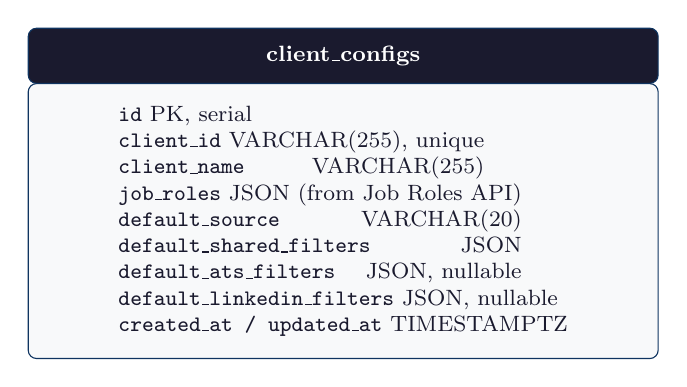
\begin{tikzpicture}[
    table/.style={rectangle, draw=accent, fill=lightbg, minimum width=8cm, align=left, font=\footnotesize, text=primary, inner sep=8pt, rounded corners=3pt},
    tablehead/.style={rectangle, draw=accent, fill=tableheader, minimum width=8cm, minimum height=0.7cm, align=center, font=\footnotesize\bfseries, text=white, inner sep=4pt, rounded corners=3pt},
]
    \node[tablehead] (ch1) {client\_configs};
    \node[table, below=-0.3pt of ch1] (ct1) {
        \texttt{id} \hfill PK, serial\\
        \texttt{client\_id} \hfill VARCHAR(255), unique\\
        \texttt{client\_name} \hfill VARCHAR(255)\\
        \texttt{job\_roles} \hfill JSON (from Job Roles API)\\
        \texttt{default\_source} \hfill VARCHAR(20)\\
        \texttt{default\_shared\_filters} \hfill JSON\\
        \texttt{default\_ats\_filters} \hfill JSON, nullable\\
        \texttt{default\_linkedin\_filters} \hfill JSON, nullable\\
        \texttt{created\_at / updated\_at} \hfill TIMESTAMPTZ
    };
\end{tikzpicture}
\end{center}

% ══════════════════════════════════════════════════════════════════════════════
\section{Error Handling}
% ══════════════════════════════════════════════════════════════════════════════

\begin{center}\small
\begin{tabularx}{\textwidth}{|L{3.5cm}|L{1.8cm}|X|}
\hline
\rowcolor{tableheader}
\textcolor{white}{\textbf{Scenario}} & \textcolor{white}{\textbf{Code}} & \textcolor{white}{\textbf{Mechanism}} \\
\hline
RapidAPI 429 & 429 & Exponential backoff (tenacity), 3 retries \\
\rowcolor{tablerow}
RapidAPI 5xx & 502 & Retry with backoff, then propagate \\
No titles + no client & 422 & Clear error message \\
\rowcolor{tablerow}
Invalid client\_id & 404 & Client not found \\
Duplicate client\_id & 409 & Conflict \\
\rowcolor{tablerow}
Both title filters set & 422 & Pydantic model\_validator \\
One source fails (both mode) & Partial & \texttt{asyncio.gather(return\_exceptions=True)} \\
\rowcolor{tablerow}
LinkedIn 7d + desc filter & Auto-fix & Auto-switch to 24h endpoint \\
\hline
\end{tabularx}
\end{center}

% ══════════════════════════════════════════════════════════════════════════════
\newpage
\section{Test Results (14/14 Passed)}
% ══════════════════════════════════════════════════════════════════════════════

All tests run against live RapidAPI with real data:

{\small
\begin{center}
\begin{tabularx}{\textwidth}{|C{0.6cm}|L{4.5cm}|C{1cm}|X|}
\hline
\rowcolor{tableheader}
\textcolor{white}{\textbf{\#}} & \textcolor{white}{\textbf{Test}} & \textcolor{white}{\textbf{Result}} & \textcolor{white}{\textbf{Details}} \\
\hline
1 & Health check & \cmark & \texttt{200 OK} \\
\rowcolor{tablerow}
2 & Onboard client with job\_roles & \cmark & \texttt{201 Created}, roles stored \\
3 & Read client config & \cmark & All data returned correctly \\
\rowcolor{tablerow}
4 & Search via client\_id (stored roles) & \cmark & 10 jobs, filter = \texttt{'Data Engineer' | 'ML Engineer' | 'Backend Developer'} \\
5 & Direct titles, no client & \cmark & 10 jobs, filter = \texttt{"Product Manager"} \\
\rowcolor{tablerow}
6 & Both sources + title override & \cmark & 19 jobs (ATS+LinkedIn), used explicit title \\
7 & ATS filters (salary + greenhouse) & \cmark & 10 jobs with real salary (\$138K--\$230K) \\
\rowcolor{tablerow}
8 & LinkedIn + seniority + UK & \cmark & 10 UK Data Scientist jobs, Mid-Senior \\
9 & No titles, no client\_id & \cmark & \texttt{422} with clear error \\
\rowcolor{tablerow}
10 & Duplicate client\_id & \cmark & \texttt{409 Conflict} \\
11 & Invalid client\_id in search & \cmark & \texttt{404 Not Found} \\
\rowcolor{tablerow}
12 & Both title filters set & \cmark & \texttt{422} validation error \\
13 & Update client job\_roles & \cmark & Roles changed to Frontend/React \\
\rowcolor{tablerow}
14 & Search after role update & \cmark & Uses new roles, returns frontend jobs \\
\hline
\end{tabularx}
\end{center}
}

% ══════════════════════════════════════════════════════════════════════════════
\section{Deployment Guide}
% ══════════════════════════════════════════════════════════════════════════════

\begin{lstlisting}[style=apistyle, title=\color{codetext}Quick Start]
cd fantastic-jobs-api
cp .env.example .env       # add RAPIDAPI_KEY
pip install -r requirements.txt
uvicorn app.main:app --reload --host 0.0.0.0 --port 8000

# Swagger UI:  http://localhost:8000/docs
# Health:      http://localhost:8000/health
\end{lstlisting}

\begin{lstlisting}[style=apistyle, title=\color{codetext}Example: Onboard Client]
POST /api/v1/clients/
{
    "client_id": "acme",
    "client_name": "Acme Corp",
    "job_roles": ["Data Engineer", "ML Engineer"],
    "default_shared_filters": {
        "location_filter": "\"United States\"",
        "remote": true, "ai_has_salary": true
    }
}
\end{lstlisting}

\begin{lstlisting}[style=apistyle, title=\color{codetext}Example: Search (using stored roles)]
POST /api/v1/search
{ "client_id": "acme", "source": "both" }
\end{lstlisting}

\begin{lstlisting}[style=apistyle, title=\color{codetext}Example: Search (direct titles)]
POST /api/v1/search
{
    "titles": ["Software Engineer", "Backend Developer"],
    "source": "ats",
    "filters": {
        "location_filter": "\"United States\"",
        "remote": true, "ai_has_salary": true
    },
    "ats_filters": { "source": ["greenhouse", "lever.co"] },
    "pagination": {"page": 1, "page_size": 50}
}
\end{lstlisting}

% ══════════════════════════════════════════════════════════════════════════════
\section{Appendix}
% ══════════════════════════════════════════════════════════════════════════════

\subsection{A. AI Taxonomy Categories (33)}

\begin{multicols}{2}
\begin{enumerate}[leftmargin=1.5em, itemsep=0pt, parsep=1pt]\small
    \item Technology \item Healthcare \item Management \& Leadership
    \item Finance \& Accounting \item Human Resources \item Sales
    \item Marketing \item Customer Service \& Support \item Education
    \item Legal \item Engineering \item Science \& Research \item Trades
    \item Construction \item Manufacturing \item Logistics
    \item Creative \& Media \item Hospitality
    \item Environmental \& Sustainability \item Retail
    \item Data \& Analytics \item Software \item Energy \item Agriculture
    \item Social Services \item Administrative
    \item Government \& Public Sector \item Art \& Design
    \item Food \& Beverage \item Transportation \item Consulting
    \item Sports \& Recreation \item Security \& Safety
\end{enumerate}
\end{multicols}

\subsection{B. Advanced Filter Operators}

\begin{center}\small
\begin{tabularx}{\textwidth}{|C{2cm}|L{2.5cm}|X|}
\hline
\rowcolor{tableheader}
\textcolor{white}{\textbf{Operator}} & \textcolor{white}{\textbf{Meaning}} & \textcolor{white}{\textbf{Example}} \\
\hline
\texttt{\&} & AND & \texttt{Python \& Django} \\
\rowcolor{tablerow}
\texttt{|} & OR & \texttt{React | Vue | Angular} \\
\texttt{!} & NOT & \texttt{Engineer \& ! Sales} \\
\rowcolor{tablerow}
\texttt{<->} & FOLLOWED BY & \texttt{Project <-> Manager} \\
\texttt{' '} & Phrase & \texttt{'Machine Learning'} \\
\rowcolor{tablerow}
\texttt{:*} & Prefix Wildcard & \texttt{Manag:*} matches Manager, Management \\
\hline
\end{tabularx}
\end{center}

\subsection{C. Seniority Levels (LinkedIn)}

Associate, Director, Executive, Mid-Senior level, Entry level, Not Applicable, Internship

\subsection{D. Work Arrangement Options}

\begin{itemize}[leftmargin=1.5em, itemsep=2pt]
    \item \textbf{On-site} -- Job is on site only, no WFH
    \item \textbf{Hybrid} -- Office with one or more remote days
    \item \textbf{Remote OK} -- Fully remote, but an office is available
    \item \textbf{Remote Solely} -- Fully remote, no office
\end{itemize}

\subsection{E. Environment Variables}

\begin{center}\small
\begin{tabularx}{\textwidth}{|L{4cm}|X|L{3cm}|}
\hline
\rowcolor{tableheader}
\textcolor{white}{\textbf{Variable}} & \textcolor{white}{\textbf{Description}} & \textcolor{white}{\textbf{Default}} \\
\hline
\texttt{RAPIDAPI\_KEY} & RapidAPI key (required) & -- \\
\rowcolor{tablerow}
\texttt{DATABASE\_URL} & DB connection string & sqlite (dev) \\
\texttt{LOG\_ENABLED} & Turn logging on/off & \texttt{true} \\
\rowcolor{tablerow}
\texttt{LOG\_LEVEL} & INFO / DEBUG / WARNING & \texttt{INFO} \\
\texttt{HTTP\_TIMEOUT} & Request timeout (seconds) & \texttt{30} \\
\rowcolor{tablerow}
\texttt{RAPIDAPI\_MAX\_CONCURRENT} & Max parallel requests & \texttt{5} \\
\hline
\end{tabularx}
\end{center}

\vfill
\begin{center}
\textcolor{highlight}{\rule{8cm}{2pt}}\\[0.5cm]
{\large\color{primary}\textbf{End of Document}}\\[0.3cm]
{\small\color{accent}Fantastic Jobs API Wrapper -- v1.0.0 -- March 2026}
\end{center}

\end{document}
